\documentclass[border=4pt]{standalone}

\usepackage{amsmath}
\usepackage{tikz}
\usepackage{mathdots}
\usepackage{yhmath}
\usepackage{cancel}
\usepackage{color}
\usepackage{siunitx}
\usepackage{array}
\usepackage{multirow}
\usepackage{amssymb}
\usepackage{gensymb}
\usepackage{tabularx}
\usepackage{booktabs}
\usetikzlibrary{fadings}
\usetikzlibrary{patterns}


\begin{document}
 




\tikzset{every picture/.style={line width=0.75pt}} %set default line width to 0.75pt        

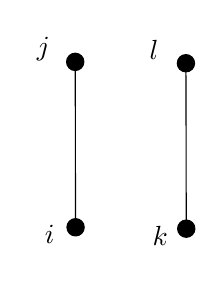
\begin{tikzpicture}[x=0.75pt,y=0.75pt,yscale=-1,xscale=1]
%uncomment if require: \path (0,300); %set diagram left start at 0, and has height of 300

%Shape: Circle [id:dp8298753983931657] 
\draw  [fill={rgb, 255:red, 0; green, 0; blue, 0 }  ,fill opacity=1 ] (91.34,170.7) .. controls (91.34,168.4) and (93.2,166.53) .. (95.5,166.53) .. controls (97.8,166.53) and (99.67,168.4) .. (99.67,170.7) .. controls (99.67,173) and (97.8,174.87) .. (95.5,174.87) .. controls (93.2,174.87) and (91.34,173) .. (91.34,170.7) -- cycle ;
%Shape: Circle [id:dp35059080828673506] 
\draw  [fill={rgb, 255:red, 0; green, 0; blue, 0 }  ,fill opacity=1 ] (91.17,91) .. controls (91.17,88.7) and (93.03,86.83) .. (95.33,86.83) .. controls (97.63,86.83) and (99.5,88.7) .. (99.5,91) .. controls (99.5,93.3) and (97.63,95.17) .. (95.33,95.17) .. controls (93.03,95.17) and (91.17,93.3) .. (91.17,91) -- cycle ;
%Straight Lines [id:da45194945483637716] 
\draw    (95.33,91) -- (95.5,170.7) ;


%Shape: Circle [id:dp16882359114705658] 
\draw  [fill={rgb, 255:red, 0; green, 0; blue, 0 }  ,fill opacity=1 ] (144.67,171.37) .. controls (144.67,169.07) and (146.53,167.2) .. (148.84,167.2) .. controls (151.14,167.2) and (153,169.07) .. (153,171.37) .. controls (153,173.67) and (151.14,175.53) .. (148.84,175.53) .. controls (146.53,175.53) and (144.67,173.67) .. (144.67,171.37) -- cycle ;
%Shape: Circle [id:dp2260640161105243] 
\draw  [fill={rgb, 255:red, 0; green, 0; blue, 0 }  ,fill opacity=1 ] (144.5,91.67) .. controls (144.5,89.37) and (146.37,87.5) .. (148.67,87.5) .. controls (150.97,87.5) and (152.83,89.37) .. (152.83,91.67) .. controls (152.83,93.97) and (150.97,95.83) .. (148.67,95.83) .. controls (146.37,95.83) and (144.5,93.97) .. (144.5,91.67) -- cycle ;
%Straight Lines [id:da003057488797083563] 
\draw    (148.67,91.67) -- (148.84,171.37) ;



% Text Node
\draw (83,174.33) node    {$i$};
% Text Node
\draw (80,84.67) node    {$j$};
% Text Node
\draw (136.33,175) node    {$k$};
% Text Node
\draw (133.33,85.33) node    {$l$};


\end{tikzpicture}

\end{document}
